%!TeX encoding = UTF-8
%!TeX program = xelatex
\documentclass[notheorems, aspectratio=54]{beamer}
% aspectratio: 1610, 149, 54, 43(default), 32

\usepackage{latexsym}
\usepackage{amsmath,amssymb}
\usepackage{mathtools}
\usepackage{color,xcolor}
\usepackage{graphicx}
\usepackage{algorithm}
\usepackage{amsthm}
\usepackage{lmodern} % 解决 font warning
% \usepackage[UTF8]{ctex}
\usepackage{animate} % insert gif

\usepackage{lipsum} % To generate test text 
\usepackage{ulem} % 下划线,波浪线
\usepackage{soul}

\usepackage{listings} % display code on slides; don't forget [fragile] option after \begin{frame}

% ----------------------------------------------
% tikx
\usepackage{framed}
\usepackage{tikz}
\usepackage{pgf}
\usetikzlibrary{calc,trees,positioning,arrows,chains,shapes.geometric,%
    decorations.pathreplacing,decorations.pathmorphing,shapes,%
    matrix,shapes.symbols}
\pgfmathsetseed{1} % To have predictable results
% Define a background layer, in which the parchment shape is drawn
\pgfdeclarelayer{background}
\pgfsetlayers{background,main}

\definecolor{AmethystPurple}{HTML}{AEAEDF}
% define styles for the normal border and the torn border
\tikzset{
  normal border/.style={AmethystPurple, decorate, 
     decoration={random steps, segment length=2.5cm, amplitude=.7mm}},
  torn border/.style={AmethystPurple, decorate, 
     decoration={random steps, segment length=.5cm, amplitude=1.7mm}}}

% Macro to draw the shape behind the text, when it fits completly in the
% page
\def\parchmentframe#1{
\tikz{
  \node[inner sep=1.5em] (A) {#1};  % Draw the text of the node
  \begin{pgfonlayer}{background}  % Draw the shape behind
  \fill[normal border] 
        (A.south east) -- (A.south west) -- 
        (A.north west) -- (A.north east) -- cycle;
  \end{pgfonlayer}}}

% Macro to draw the shape, when the text will continue in next page
\def\parchmentframetop#1{
\tikz{
  \node[inner sep=2em] (A) {#1};    % Draw the text of the node
  \begin{pgfonlayer}{background}    
  \fill[normal border]              % Draw the ``complete shape'' behind
        (A.south east) -- (A.south west) -- 
        (A.north west) -- (A.north east) -- cycle;
  \fill[torn border]                % Add the torn lower border
        ($(A.south east)-(0,.2)$) -- ($(A.south west)-(0,.2)$) -- 
        ($(A.south west)+(0,.2)$) -- ($(A.south east)+(0,.2)$) -- cycle;
  \end{pgfonlayer}}}

% Macro to draw the shape, when the text continues from previous page
\def\parchmentframebottom#1{
\tikz{
  \node[inner sep=2em] (A) {#1};   % Draw the text of the node
  \begin{pgfonlayer}{background}   
  \fill[normal border]             % Draw the ``complete shape'' behind
        (A.south east) -- (A.south west) -- 
        (A.north west) -- (A.north east) -- cycle;
  \fill[torn border]               % Add the torn upper border
        ($(A.north east)-(0,.2)$) -- ($(A.north west)-(0,.2)$) -- 
        ($(A.north west)+(0,.2)$) -- ($(A.north east)+(0,.2)$) -- cycle;
  \end{pgfonlayer}}}

% Macro to draw the shape, when both the text continues from previous page
% and it will continue in next page
\def\parchmentframemiddle#1{
\tikz{
  \node[inner sep=2em] (A) {#1};   % Draw the text of the node
  \begin{pgfonlayer}{background}   
  \fill[normal border]             % Draw the ``complete shape'' behind
        (A.south east) -- (A.south west) -- 
        (A.north west) -- (A.north east) -- cycle;
  \fill[torn border]               % Add the torn lower border
        ($(A.south east)-(0,.2)$) -- ($(A.south west)-(0,.2)$) -- 
        ($(A.south west)+(0,.2)$) -- ($(A.south east)+(0,.2)$) -- cycle;
  \fill[torn border]               % Add the torn upper border
        ($(A.north east)-(0,.2)$) -- ($(A.north west)-(0,.2)$) -- 
        ($(A.north west)+(0,.2)$) -- ($(A.north east)+(0,.2)$) -- cycle;
  \end{pgfonlayer}}}

% Define the environment which puts the frame
% In this case, the environment also accepts an argument with an optional
% title (which defaults to ``Example'', which is typeset in a box overlaid
% on the top border
\newenvironment{parchment}[1][Example]{%
  \def\FrameCommand{\parchmentframe}%
  \def\FirstFrameCommand{\parchmentframetop}%
  \def\LastFrameCommand{\parchmentframebottom}%
  \def\MidFrameCommand{\parchmentframemiddle}%
  \vskip\baselineskip
  \MakeFramed {\FrameRestore}
  \noindent\tikz\node[inner sep=1ex, draw=black!20,fill=AmethystPurple, 
          anchor=west, overlay] at (0em, 1em) {\sffamily#1};\par}%
{\endMakeFramed}

% ----------------------------------------------

\mode<presentation>{
    \usetheme{Berkeley}
    % Boadilla CambridgeUS
    % default Antibes Berlin Copenhagen
    % Madrid Montpelier Ilmenau Malmoe
    % Berkeley Singapore Warsaw
    \usecolortheme{dolphin}
    % beetle, beaver, orchid, whale, dolphin
    \useoutertheme{infolines}
    % infolines miniframes shadow sidebar smoothbars smoothtree split tree
    \useinnertheme{circles}
    % circles, rectanges, rounded, inmargin
}
% 设置 block 颜色
\setbeamercolor{block title}{bg=AmethystPurple,fg=white}

\newcommand{\reditem}[1]{\setbeamercolor{item}{fg=red}\item #1}

% 缩放公式大小
\newcommand*{\Scale}[2][4]{\scalebox{#1}{\ensuremath{#2}}}

% 解决 font warning
\renewcommand\textbullet{\ensuremath{\bullet}}

% ---------------------------------------------------------------------
% flow chart
\tikzset{
    >=stealth',
    punktchain/.style={
        rectangle, 
        rounded corners, 
        % fill=black!10,
        draw=white, very thick,
        text width=6em,
        minimum height=2em, 
        text centered, 
        on chain
    },
    largepunktchain/.style={
        rectangle,
        rounded corners,
        draw=white, very thick,
        text width=10em,
        minimum height=2em,
        on chain
    },
    line/.style={draw, thick, <-},
    element/.style={
        tape,
        top color=white,
        bottom color=blue!50!black!60!,
        minimum width=6em,
        draw=blue!40!black!90, very thick,
        text width=6em, 
        minimum height=2em, 
        text centered, 
        on chain
    },
    every join/.style={->, thick,shorten >=1pt},
    decoration={brace},
    tuborg/.style={decorate},
    tubnode/.style={midway, right=2pt},
    font={\fontsize{10pt}{12}\selectfont},
}
% ---------------------------------------------------------------------

% code setting
\lstset{
    language=C++,
    basicstyle=\ttfamily\footnotesize,
    keywordstyle=\color{red},
    breaklines=true,
    xleftmargin=2em,
    numbers=left,
    numberstyle=\color[RGB]{222,155,81},
    frame=leftline,
    tabsize=4,
    breakatwhitespace=false,
    showspaces=false,               
    showstringspaces=false,
    showtabs=false,
    morekeywords={Str, Num, List},
}

% ---------------------------------------------------------------------

%% preamble
\title[Testing Vendor Android as a Service-Oriented System]{Testing Vendor Android as a Service-Oriented System}
% \subtitle{The subtitle}
\author{Xiangsen Liao}
\institute[ICS] % (optional)
{
	Institute of Computer Software\\
	Nanjing University
}

\date[Report 2020.10] % (optional)
{I2EC Report, Nov 2020}

% -------------------------------------------------------------

\begin{document}

%% title frame
\begin{frame}
    \titlepage
\end{frame}

%% normal frame
\section{Background}

\begin{frame}
	
	\begin{block}{Understand Vendor Customizations}
		On the Kernel layer, changes mainly happen to the \textcolor{red}{driver and arch} dirctory; on the Framework layer, most of the customizations are either related to \textcolor{red}{custom device or pre-installed Applications}.
		\begin{figure}
			\centering
			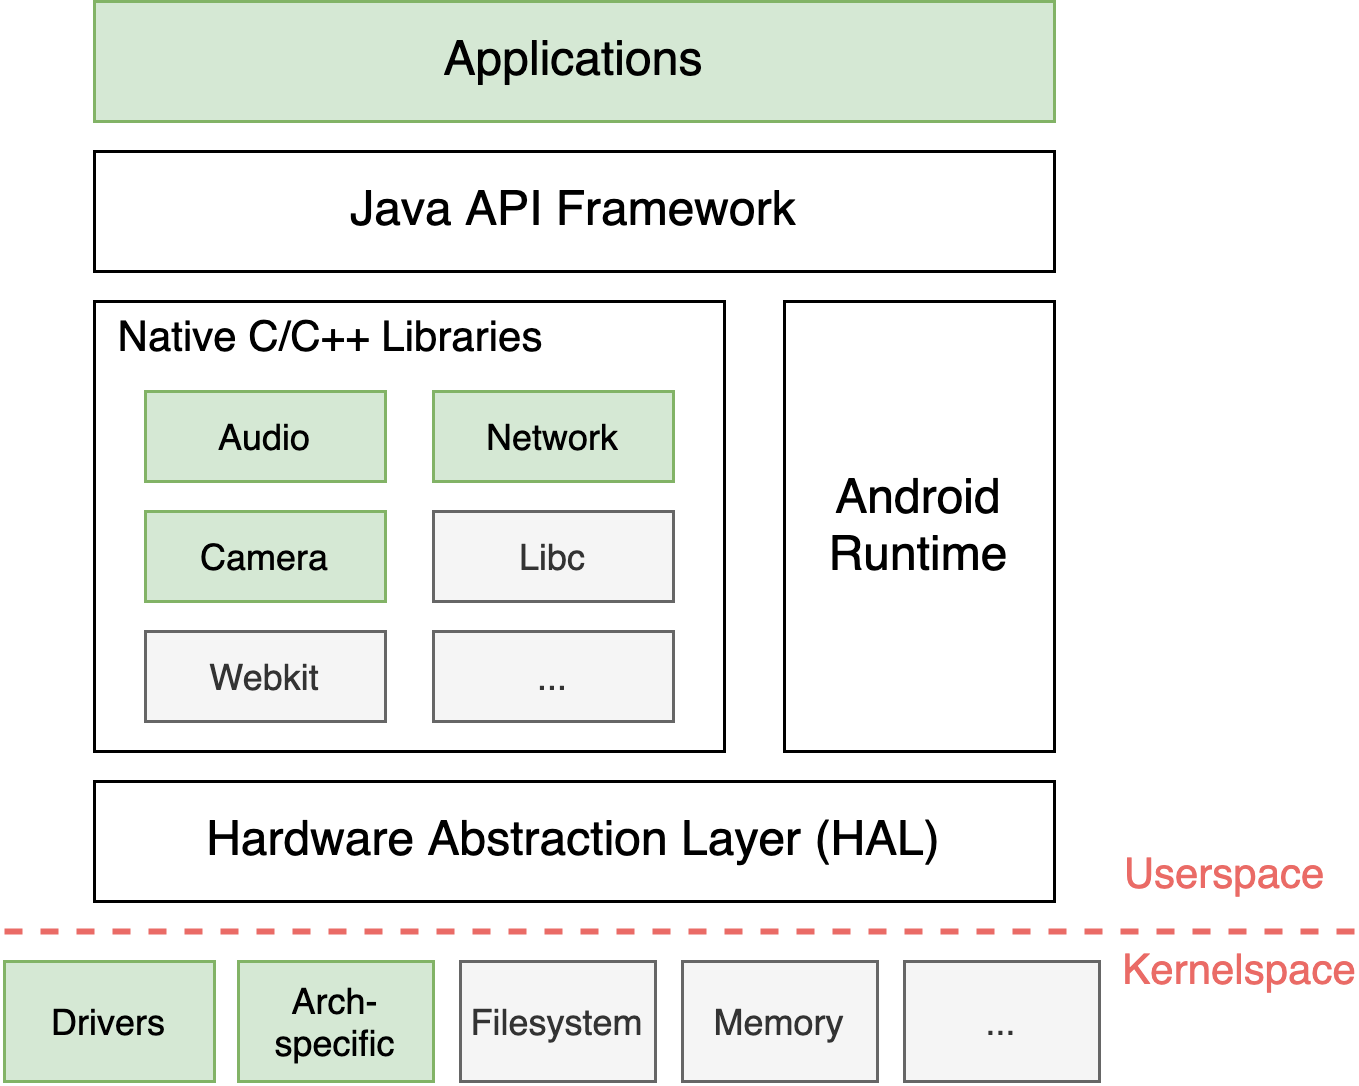
\includegraphics[width=0.6\textwidth]{res/Android-layers.png}
			\vspace*{-0.2cm}
		\end{figure}
	\end{block}

\end{frame}

\begin{frame}

	\begin{block}{Security Risks in Vendor Android Customization}
		Previous works\footnote{\tiny{Harvesting Inconsistent Security Configurations in Custom Android ROMs via Differential Analysis, USENIX Security 16}} \footnote{\tiny{An Analysis of Pre-installed Android Software, S\&P 20}} has proved that Android vendor customization could be problematic. 
		\\[2ex]
		Case Study on Android root exploits show\footnote{\tiny{Android Root and its Providers: A Double-Edged Sword, CCS 15}}: most of vulnerabilities are introduced by \textcolor{red}{vendor customization} at the \textcolor{red}{External Drivers and Application Layer}.
		\begin{figure}
			\centering
			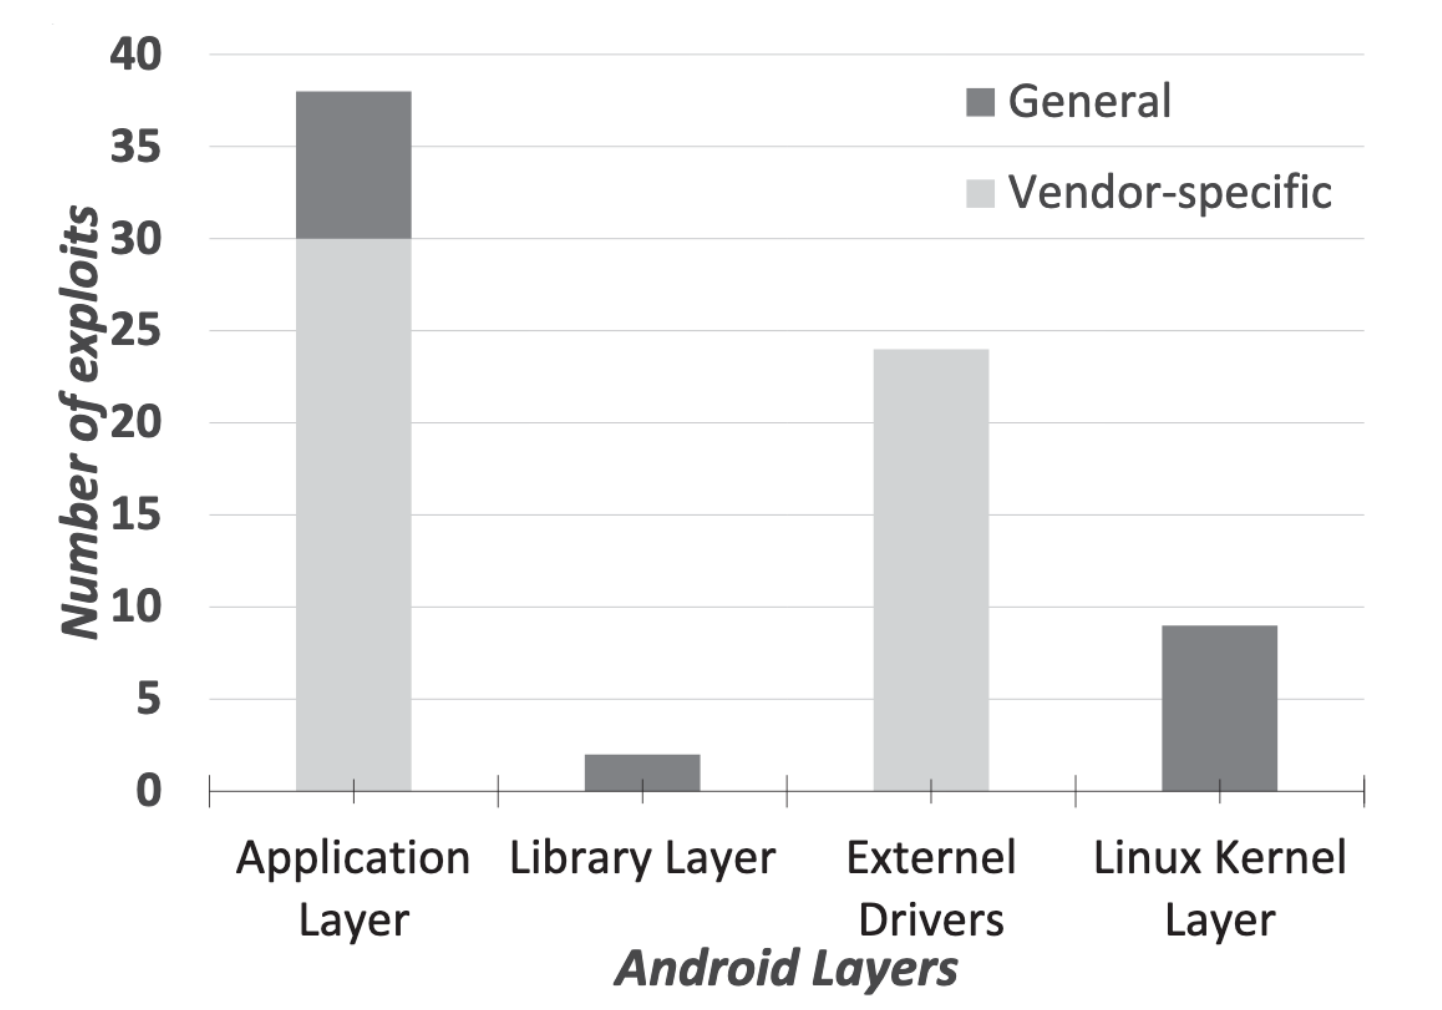
\includegraphics[width=0.55\textwidth]{res/exploits-category-before-2015.png}
			\vspace*{-0.3cm}
		\end{figure}
	\end{block}

\end{frame}


\section{Why Focus on Service?}

\begin{frame}

    \begin{block}{Android Framework is a Service-Oriented System}
     	Unlike the Linux kernel, which stores most information of a process in \textcolor{red}{a centralized structure "task\_struct"}. 
     	\\[2ex]
     	Android Framework code is structured as \textcolor{red}{a set of system service classes}, each of which points to some objects and arrays for storing app-specific information.
    \end{block}

	\begin{block}{Service has Large Attack Surface}
		Vendor Android bring more Services than AOSP:
		\begin{itemize}
			\item Over 150 vendor Services in MIUI-10.0 OS (Android 8.0)
			\item Over 100 vendor Services in Samsung OS (Android 10.0)
		\end{itemize}
	\end{block}

	\begin{block}{Service is Worth to Attack}
		\begin{itemize}
			\item Most of them are running in privileged process
			\item Full access to hardware resource
		\end{itemize}
	\end{block}

\end{frame}

\section{Challenge}

\begin{frame}
	\begin{block}{Vendor Android System is Close-sourced}
		 Vendor providers just need to open-source custom Kernel.
		 % \\[1ex]
		 % Vendor Android can't run on emulator, so we need to impl Testing Tracing 
		 \\[1ex]
		 Brute force black-box Testing is ineffective, we need to extract type information of Android Service without source code.
	\end{block}

	\begin{block}{Hard to Metric Testing Tools}
		Previous works collect code/method coverage by Java/Bytecode Instrumentation. 
		\\[1ex]
		For close-sourced vendor Android System, we can only collect block coverage by Binary Instrumentation.
	\end{block}
\end{frame}


\section{Case Study: Service Bugs}

\if fasle
\begin{frame}
	
	Collect from Android security bulletin\footnote{\tiny{https://source.android.com/security/bulletin}}, case study of patch code commit in AOSP.
	
	\begin{block}{Inconsistent Serialization}
		2018-05 bulletin, CVE-2017-13315. IPC contains custom Parcelable Object, requires \textcolor{red}{\texttt{writeToParcel()} and \texttt{readFromParcel()} to be symmetric}.
		
		In this case, a long integer is serialized but a normal interger is deserialized.
		\begin{figure}
			\centering
			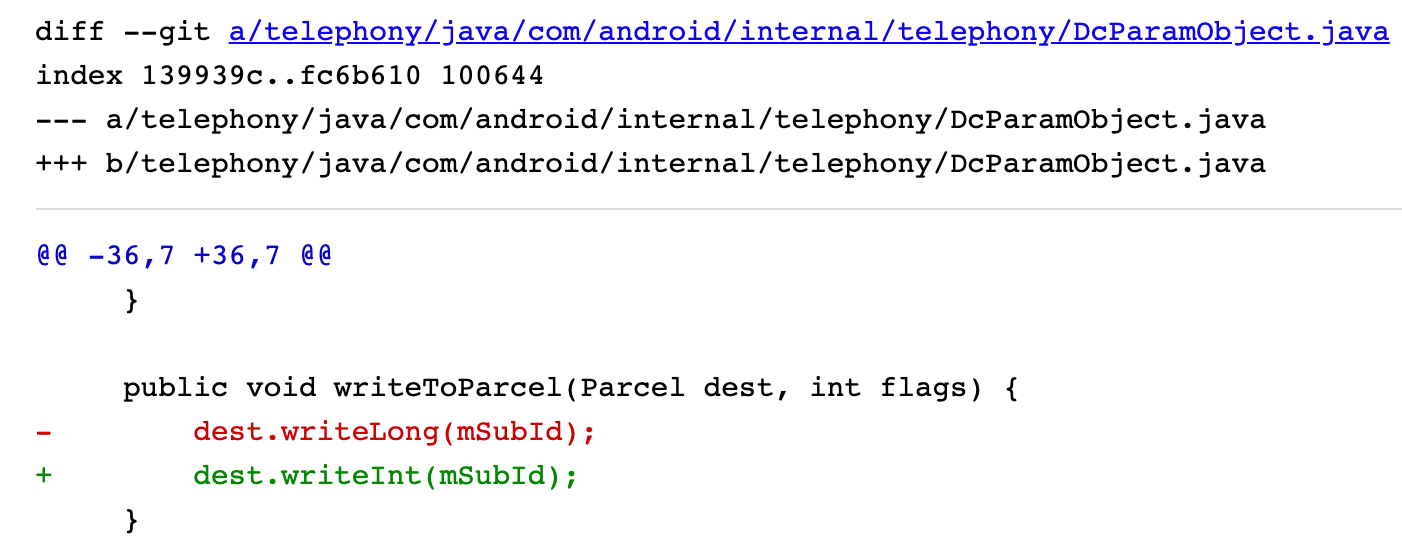
\includegraphics[width=0.95\textwidth]{res/case-study-inconsistent-serialization.png}
			\vspace*{-0.3cm}
		\end{figure}
	\end{block}

	How to reproduce: generate boundary value.
	
\end{frame}
\fi

\begin{frame}
	
	Bugs are collect from \textcolor{red}{Android Security Bulletin}\footnote{\tiny{https://source.android.com/security/bulletin}}, case study of patch code commit.
	\\[2ex]
	Try to understand Android Service Bugs, and find how to reproduce similar Bugs.  
\end{frame}

\begin{frame}
	\begin{block}{Inconsistent Serialization}
		2018-05 bulletin, CVE-2017-13315
		\\[1ex]
		\scriptsize{IPC contains custom Parcelable Object, requires \textcolor{red}{\texttt{writeToParcel()} and \texttt{readFromParcel()} to be symmetric}. In this case, a long integer is serialized but a normal interger is deserialized.}
		
		\begin{figure}
			\centering
			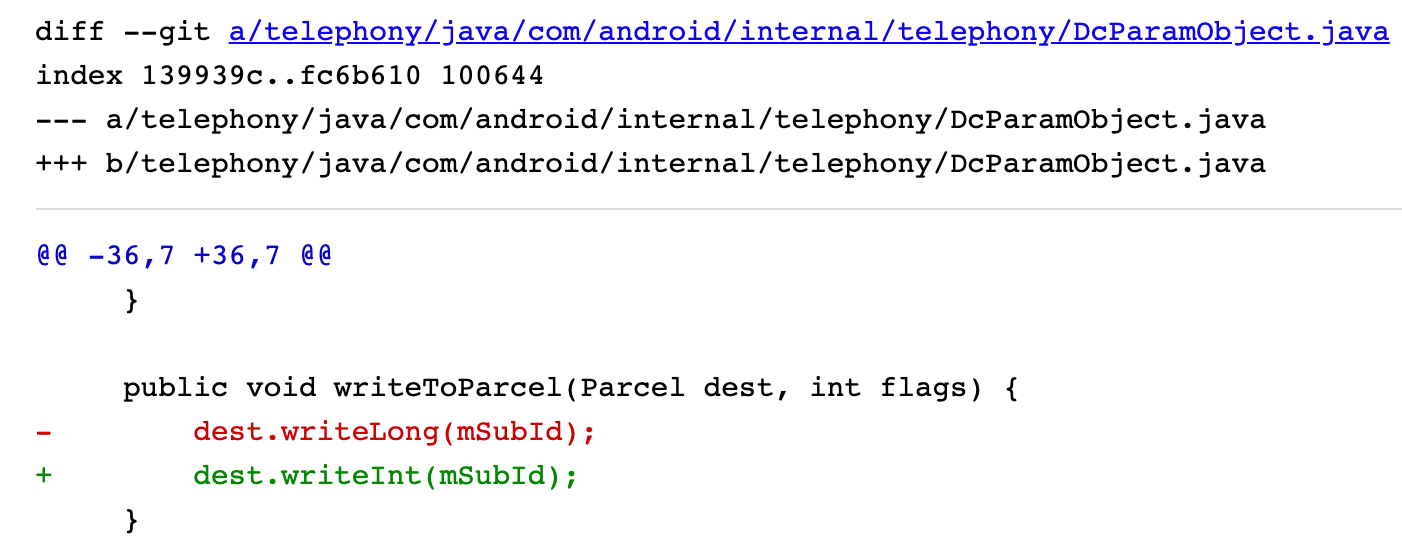
\includegraphics[width=0.95\textwidth]{res/case-study-inconsistent-serialization.png}
			\vspace*{-0.3cm}
		\end{figure}
	\end{block}
	
	How to reproduce: generate boundary value.
	
\end{frame}

\begin{frame}
	\begin{block}{Keep Reference of a Dead Service}
		2017-04 bulletin, CVE-2017-0544
		\\[1ex]
		\scriptsize{If \texttt{CameraService} dies, Binder death callback will clear the \texttt{gCameraService}(a pointer wrapper to \texttt{CameraService})} automatically, this means \texttt{gCameraService} will point to NULL. 
		 
		If \texttt{getCameraService()} return the reference to \texttt{gCameraService}, caller may keep a \textcolor{red}{NULL pointer wrapper when \texttt{CameraService} died}.
		
		\begin{figure}
			\centering
			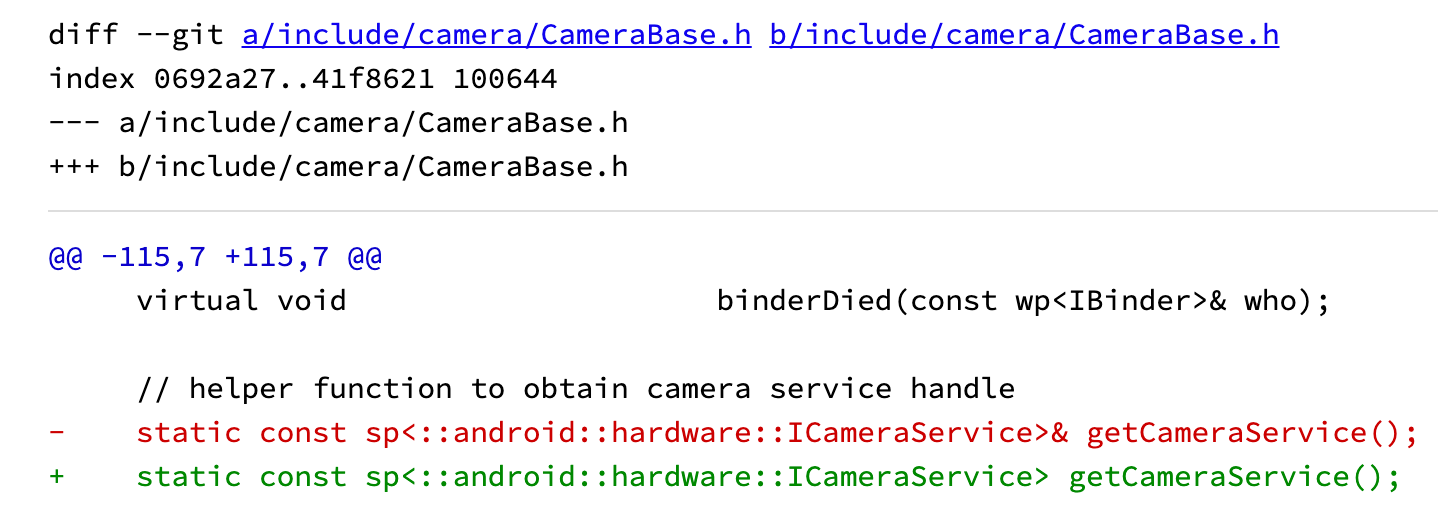
\includegraphics[width=0.95\textwidth]{res/case-study-reference-to-dead-service.png}
			\vspace*{-0.3cm}
		\end{figure}
	\end{block}

	How to reproduce: kill dependent Service when Service IPC execution.

\end{frame}


\section{Binder IPC Internal}

\begin{frame}
	
	\textbf{Binder IPC from Developer View:} 
	
	Android SDK will generate \textcolor{red}{Java/C++ Stub code} from AIDL\footnote{\tiny{https://developer.android.com/guide/components/aidl}}(Android Interface Definition Language).
	
	\begin{columns}
		\begin{column}{0.2\textwidth}
			\scriptsize{IRemoteService.aidl}
		\end{column}
		\begin{column}{0.7\textwidth}
			\begin{figure}
				\begin{flushleft}
					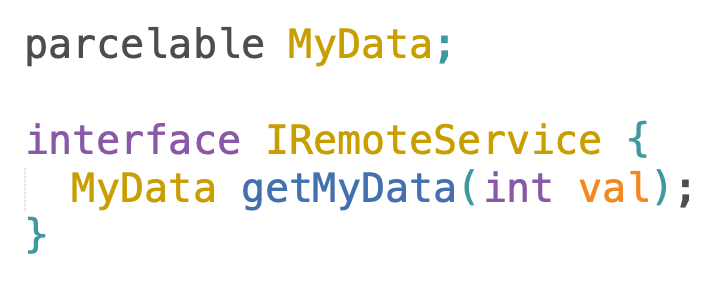
\includegraphics[width=0.40\textwidth]{res/aidl-example.png}
				\end{flushleft}
			\end{figure}
		\end{column}
	\end{columns}
	
	\begin{columns}
		\begin{column}{0.2\textwidth}
			\scriptsize{ExampleClient.java}
		\end{column}
		\begin{column}{0.7\textwidth}
			\begin{figure}
				\begin{flushleft}
				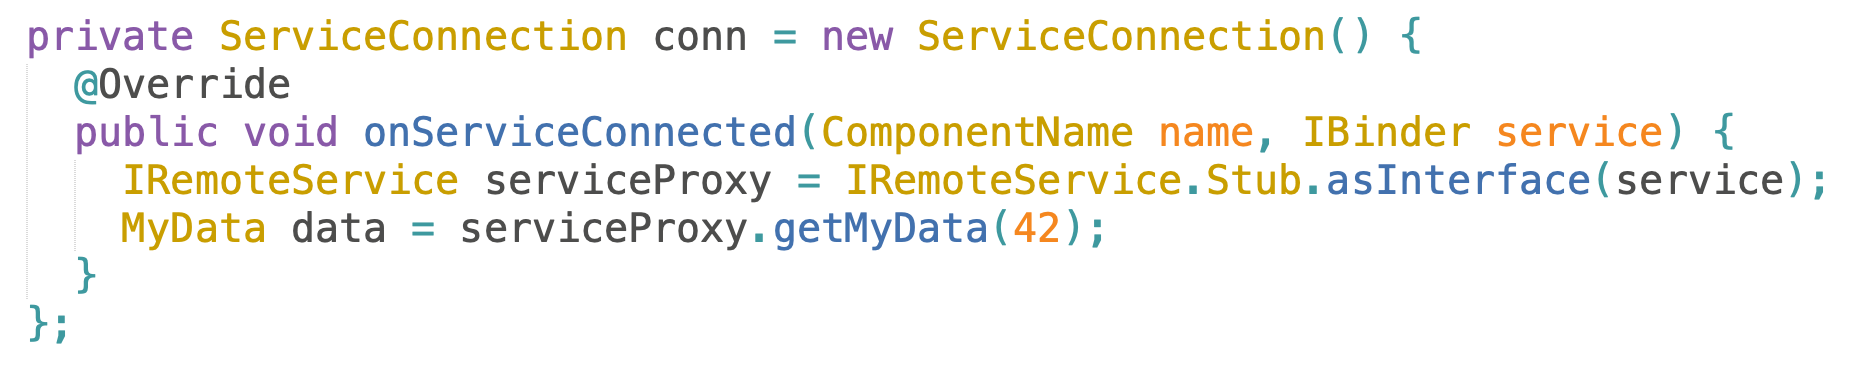
\includegraphics[width=\textwidth]{res/aidl-example-client.png}
				\end{flushleft}
			\end{figure}
		\end{column}
	\end{columns}

	\begin{columns}
		\begin{column}{0.2\textwidth}
			\scriptsize{ExampleServer.java}
		\end{column}
		\begin{column}{0.7\textwidth}
			\begin{figure}
				\begin{flushleft}
				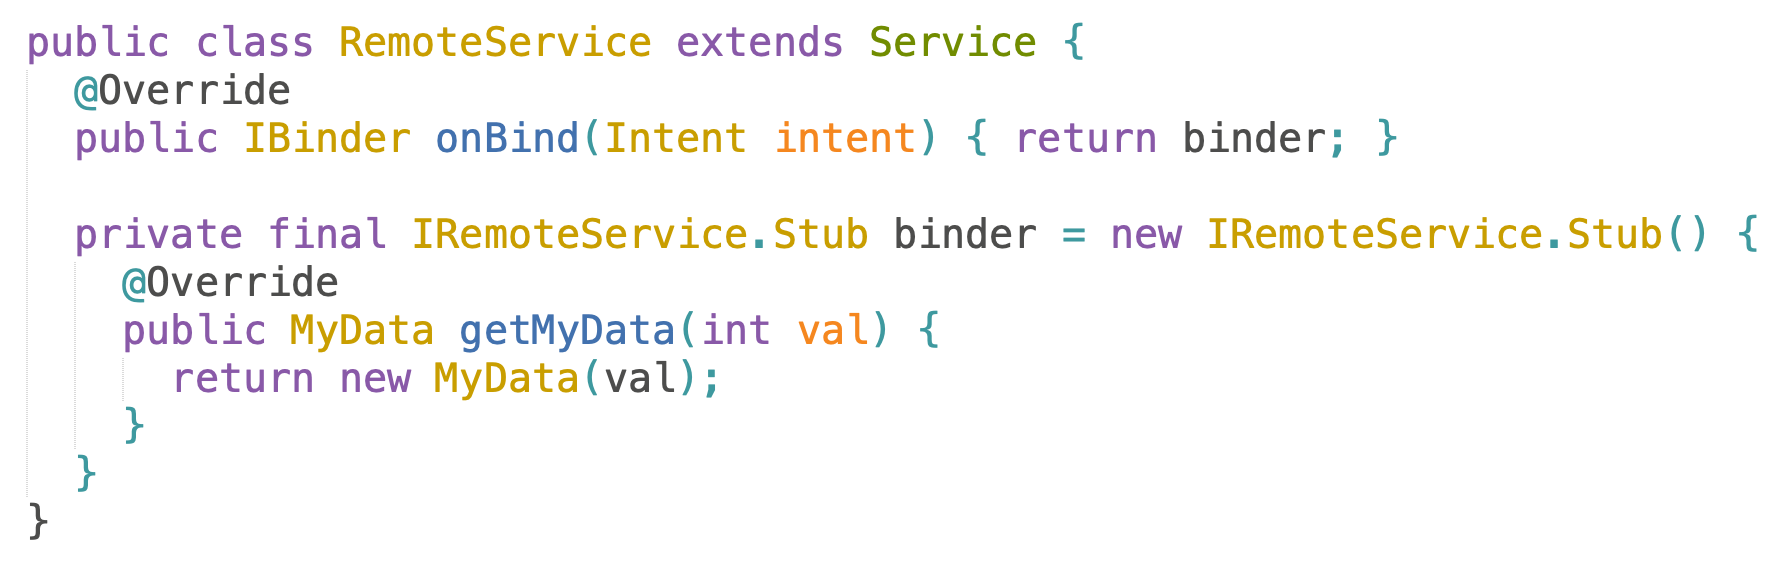
\includegraphics[width=\textwidth]{res/aidl-example-server.png}
				\end{flushleft}
			\end{figure}
		\end{column}
	\end{columns}
\end{frame}

\begin{frame}
	
	This \textcolor{red}{auto-generated \texttt{ServiceStub} Smali code} is extracted from MIUI-10 ROM. 
	
	The \texttt{MiuiPerfService} is running in \texttt{Process(com.miui.daemon)}, we only focus on method \texttt{onTransact()}.
	
	\begin{columns}
		\begin{column}{0.2\textwidth}
			\\[6ex]
			\tiny{
				WriteServiceDescriptor
				\\[2ex]
				return True
			}
			\\[4ex]
			\tiny{
				MethodID is 0x4
				
				Parcel.readxxx()
				DoSomething()
				Parcel.writexxx()
			}
			\\[4ex]
			\tiny{
				Switch-Case depends on \texttt{MethodID}
			}
		\end{column}
		\begin{column}{0.8\textwidth}
			\begin{figure}
				\begin{flushleft}
					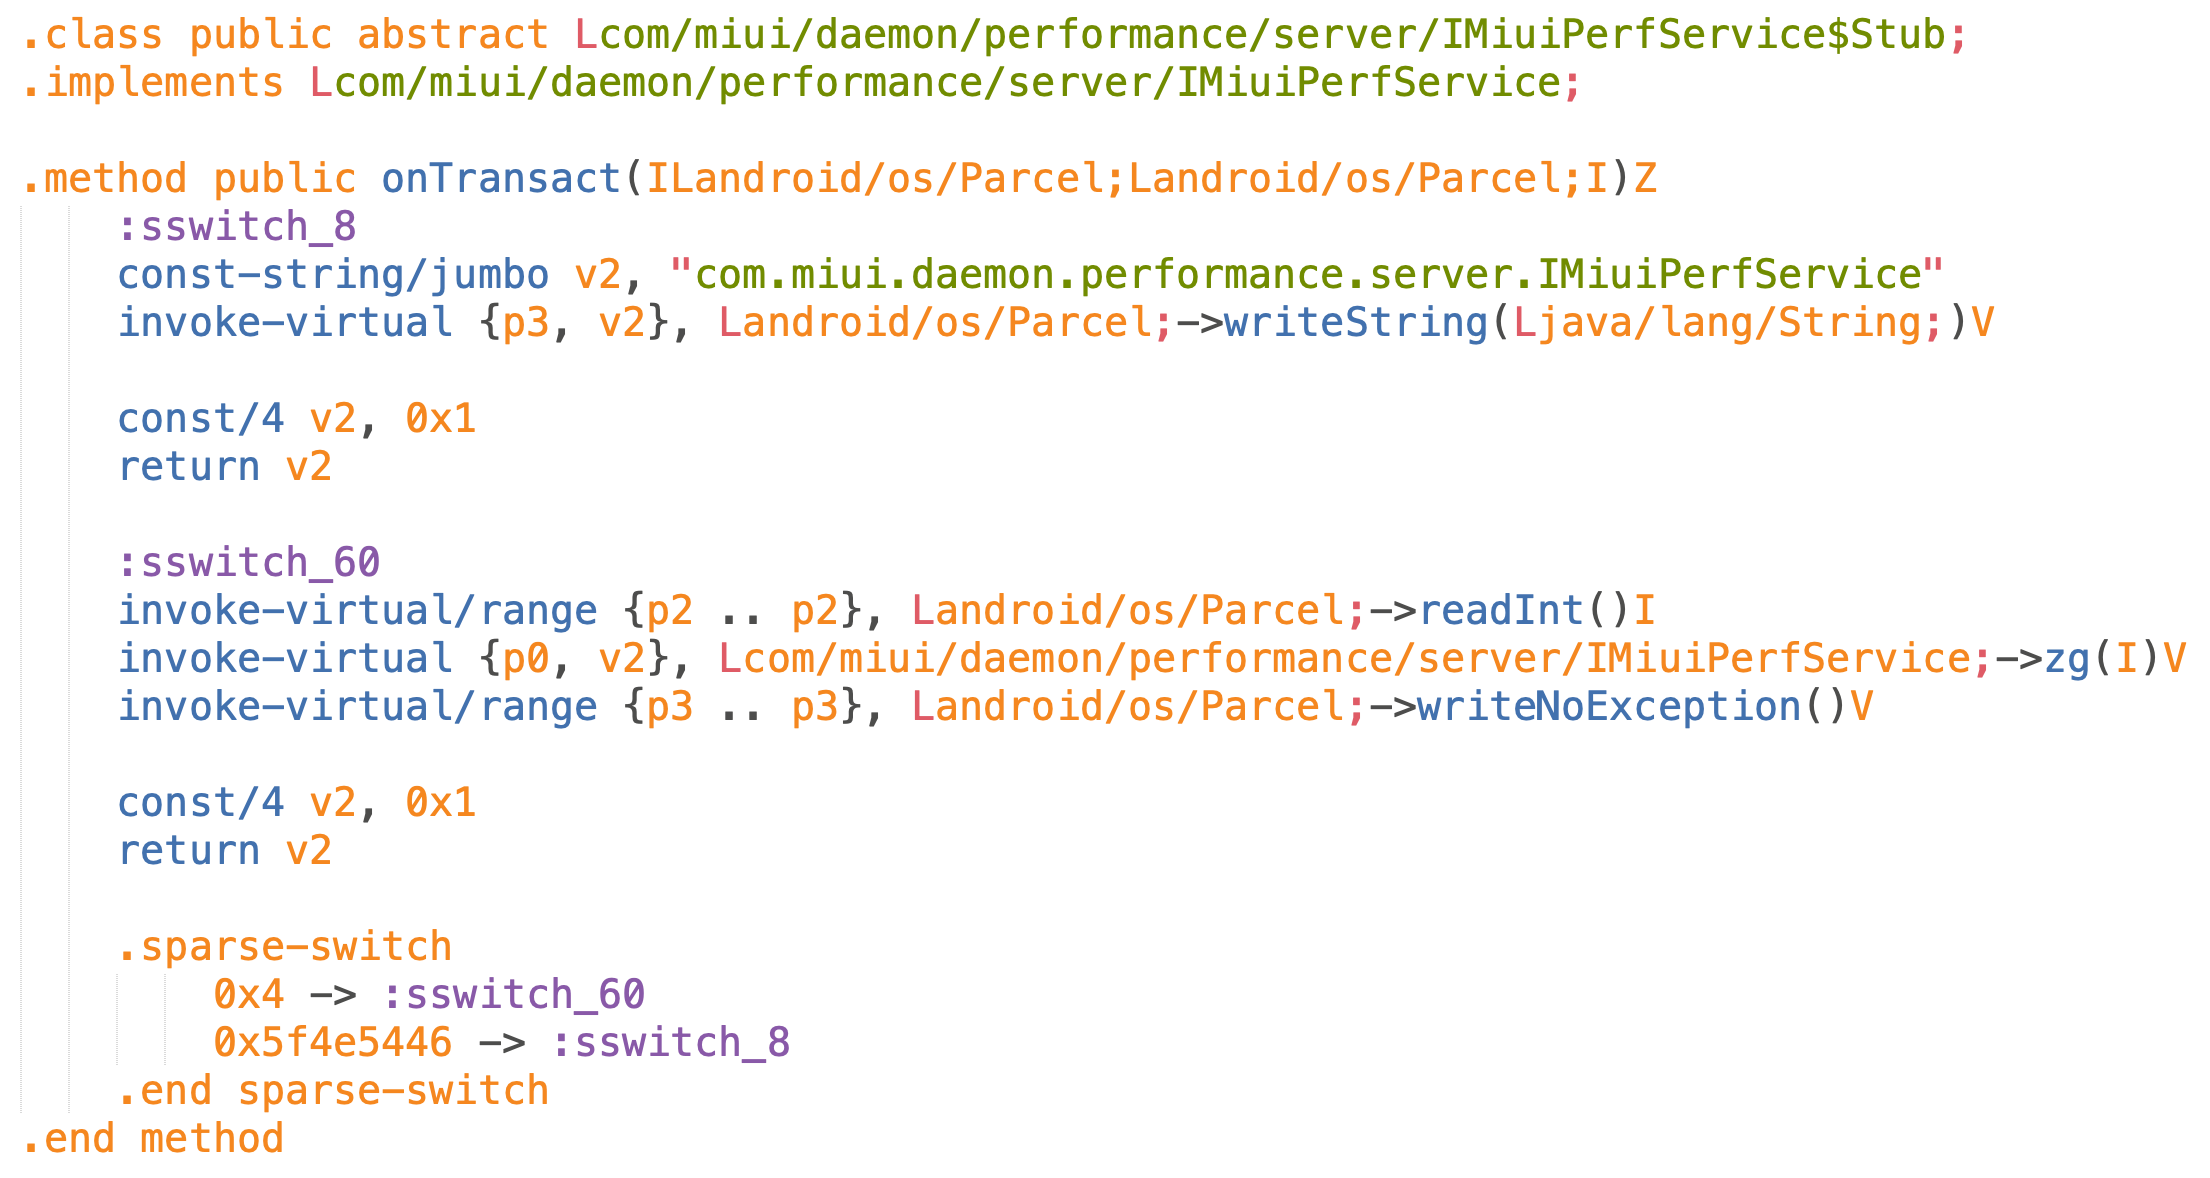
\includegraphics[width=\textwidth]{res/aidl-example-stub.png}
				\end{flushleft}
			\end{figure}
		\end{column}
	\end{columns}
	
	With this knowledge, \textcolor{red}{we can extract Service Method Signature from a vendor ROM.} 

\end{frame}


\begin{frame}
	
	\textbf{Binder IPC from Kernel View:}
	
	Just \texttt{Ioctl(2)} system call. 
	
	\begin{figure}
		\centering
		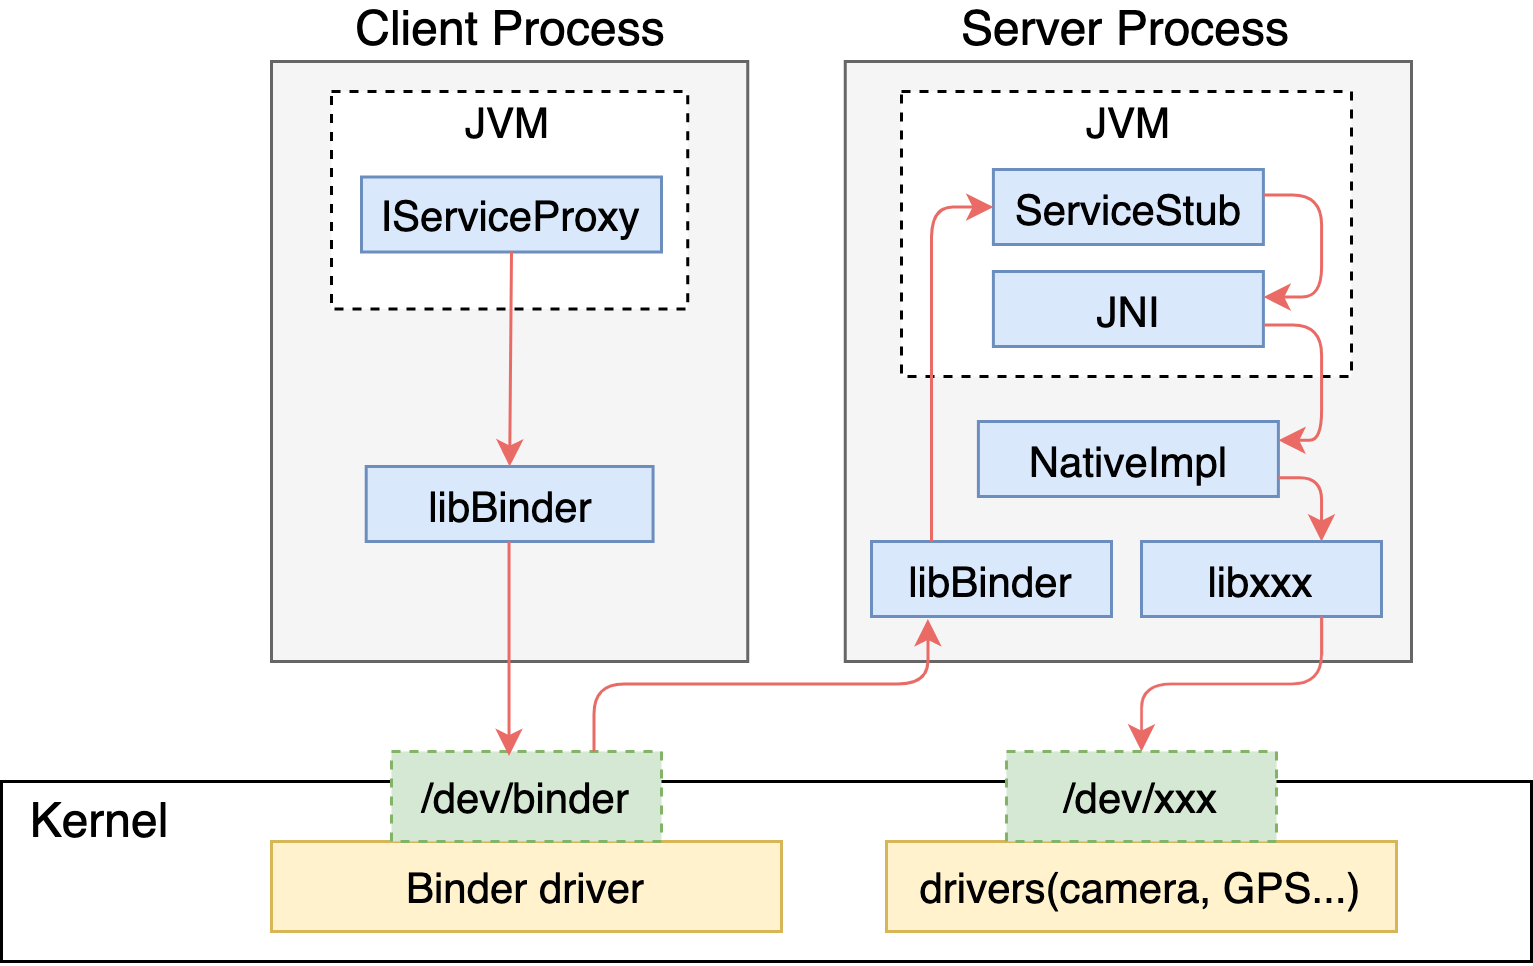
\includegraphics[width=\textwidth]{res/binder-internal.png}
	\end{figure}

\end{frame}

\begin{frame}
	
	With \textcolor{red}{the Kernel structure definition in Binder driver}, we can parse IPC information(PID, ServiceName, MethodID) from \texttt{Ioctl(2)} param.
	
	\begin{figure}
		\centering
		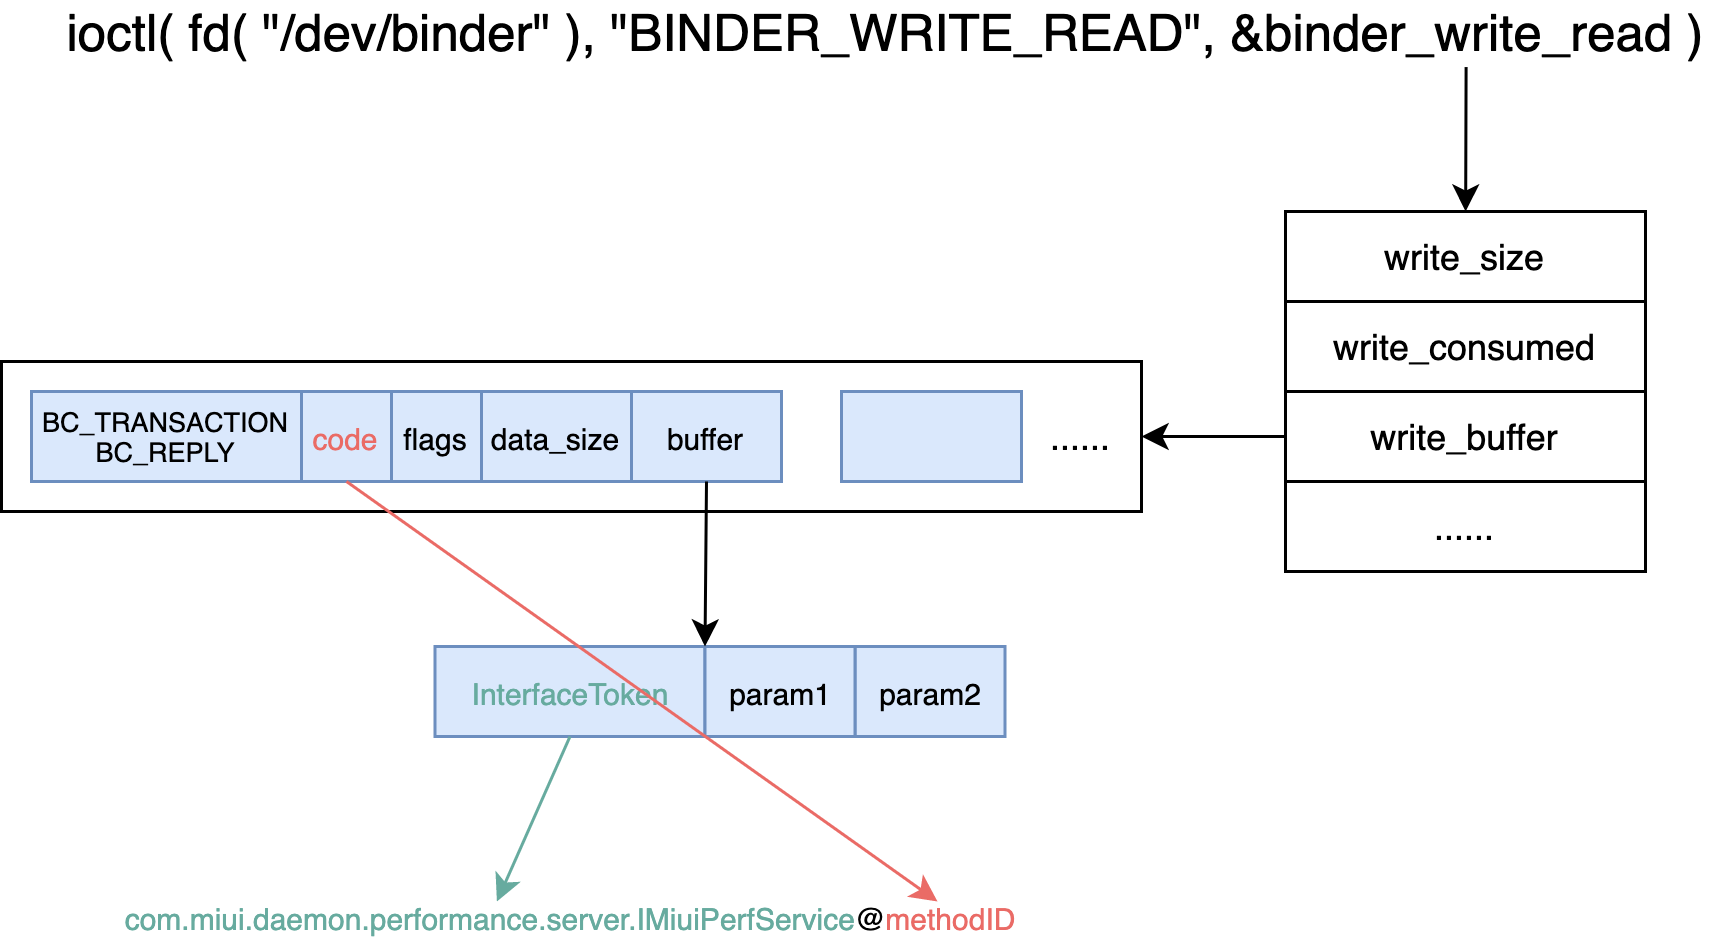
\includegraphics[width=\textwidth]{res/binder-structure.png}
	\end{figure}
	
	With this knowledge, \textcolor{red}{we can intercept Binder system call to manipulate IPC request and reply.} 
\end{frame}


\section{How to Manipulate Service IPC}
\begin{frame}

	\textbf{Related works:}
	
	Testing Android Application and System at Inter-Component Communication level, most of the works focus on Application.

	\begin{block}{Manipulation at Intent Level}
		Focus on how to generate \texttt{Action(constant)} and \texttt{Extras(key-value)}.
		\begin{itemize}
			\item IntentFuzzer\footnote{\tiny{IntentFuzzer: detecting capability leaks of android applications, AsiaCCS 14}}: focus on permission leaks(miss Permission/UID check, mis-exported component).
			\item Snowdrop\footnote{\tiny{Systematically testing background services of mobile apps, ASE 17}}: guess \texttt{Extras.value} from source code, and mock Android Framework API to return malformed hardware state.
		\end{itemize}
	\end{block}
\end{frame}

\begin{frame}
	Intent limitaion: Android NDK(\textcolor{red}{over 35\% Services are impl in C++ on MIUI-10}) don't support Intent, most of the System Services talk to each other use AIDL directly.

	\begin{block}{Manipulation at AIDL/Binder level}
		\begin{itemize}
			\item BinderCracker\footnote{\tiny{Assessing the Robustness of Android System Services, 16}}: black-box, record Binder transaction, mutate the parameters and replay.
			\item Chizpurfle\footnote{\tiny{A Gray-Box Android Fuzzer for Vendor Service Customizations, ISSRE 17}}: grey-box, focus on Java Service, extract Method Signature by reflection and fuzzing params.
			\item FANS\footnote{\tiny{Fuzzing Android Native System Services via Automated Interface Analysis, USENIX Security 20}}: white-box, program analysis of AIDL source code in AOSP.
		\end{itemize}
	\end{block}
	
\end{frame}

\begin{frame}
	\textbf{Approach:}
	\begin{itemize}
		\item primitive type and custom structure: randomly mutate the bytes, generate boundary value.
		\item remote reference(other service or callback): pass a dead service reference; pass malformed callback(long running or throw uncaughted Exception).
		\item execution context: malformed hardware related system call.
	\end{itemize}
\end{frame}

\section{How to Guide Testing}
\begin{frame}
	
	\textbf{Is Crash Detection Enough?}
	
	The efficiency of Crash detection is a widely used assessment metric. But it might not be suitable for Testing Android Service.
	
	\begin{block}{Android Service Design Philosophy: Let it Restart}
		Over 150 Services in Process(\texttt{system\_server}) on MIUI-10.
		
		Process(\texttt{system\_server}) will \textcolor{red}{kill itself when any Service Blocked or Crashed(soft-reboot).}
		
		Most of the Services are safe to Crash and Restart in Android Framework. 
	\end{block}
\end{frame}

\begin{frame}
	\begin{figure}
		\centering
		
\includegraphics[width=0.9\textwidth]{res/thanks.pdf}
	\end{figure}
\end{frame}

\end{document}